% !TeX root = ./ms.tex
\documentclass[modern]{aastex62}

% Load the corTeX style definitions
% !TeX root = ./ms.tex
% All the packages
\usepackage{url}
\usepackage{amsmath}
\usepackage{mathtools}
\usepackage{amssymb}
\usepackage{natbib}
\usepackage{graphicx}
\usepackage{calc}
\usepackage{etoolbox}
\usepackage{xspace}
\usepackage[T1]{fontenc} % https://tex.stackexchange.com/a/166791
\usepackage{textcomp}
\usepackage{ifxetex}
\ifxetex
  \usepackage{fontspec}
  \defaultfontfeatures{Extension = .otf}
\fi
\usepackage{fontawesome}
\usepackage{listings}
\usepackage{nicefrac}
\usepackage[bb=boondox]{mathalfa}
\usepackage{booktabs}
\usepackage{longtable}

% Shorthand for this paper
\newcommand{\starry}{\textsf{starry}\xspace}
\newcommand{\Python}{\textsf{Python}\xspace}
\newcommand{\cpp}{\textsf{C}++\xspace}
\newcommand{\bvec}[1]{{\ensuremath{\mathbf{#1}}}}
\newcommand{\xxx}[1]{{\color{red}#1}}
\DeclarePairedDelimiter\floor{\lfloor}{\rfloor}
\DeclarePairedDelimiter\ceil{\lceil}{\rceil}
\newcommand{\imag}{{\ensuremath{\mathbb{i}}}}
\newcommand{\quadquad}{\quad\quad\quad\quad}

\newcommand{\R}{\bvec{R}}
\newcommand{\AOne}{\bvec{A_1}}
\newcommand{\alm}{\bvec{a}}
\newcommand{\x}{\bvec{x}}
\newcommand{\D}{D}
\newcommand{\Doppler}{\bvec{D}}
\newcommand{\Surf}{\mathcal{S}}
\newcommand{\Curve}{\mathcal{C}}
\newcommand{\Dargs}{\bvec{d}}
\newcommand{\lmax}{\ensuremath{l_\mathrm{max}}}
\newcommand{\spot}{\texttt{SPOT}\xspace}
\newcommand{\vogtstar}{\texttt{VOGTSTAR}\xspace}
\newcommand{\kT}{\boldsymbol{\kappa}^\top}
\newcommand{\rhoT}{\boldsymbol{\rho}^\top}
\newcommand{\ylmbasis}{\boldsymbol{\psi}^\top}
\newcommand{\pbasis}{\boldsymbol{\phi}^\top}
\newcommand{\pbasisn}{\ensuremath{\phi_n}}
\newcommand{\azero}{\ensuremath{\bvec{a_0}}}

% References to text content
\newcommand{\documentname}{\textsl{article}}
\newcommand{\figureref}[1]{\ref{fig:#1}}
\newcommand{\Figure}[1]{Figure~\figureref{#1}}
\newcommand{\figurelabel}[1]{\label{fig:#1}}
\renewcommand{\eqref}[1]{\ref{eq:#1}}
\newcommand{\Eq}[1]{Equation~(\eqref{#1})}
\newcommand{\eq}[1]{\Eq{#1}}
\newcommand{\eqalt}[1]{Equation~\eqref{#1}}

% Add code, proof, and animation hyperlinks
\definecolor{linkcolor}{rgb}{0.1216,0.4667,0.7059}
\newcommand{\codeicon}{{\color{linkcolor}\faFileCodeO}}
\newcommand{\prooficon}{{\color{linkcolor}\faPencilSquareO}}
\newcommand{\codelink}[1]{\href{https://github.com/user/repo/blob/fe12fa16a5cc76c1ba72d97241fb9545da144edf/tex/figures/#1.py}{\codeicon}\,\,}
\newcommand{\animlink}[1]{\href{https://github.com/user/repo/blob/fe12fa16a5cc76c1ba72d97241fb9545da144edf/tex/figures/#1.gif}{\animicon}\,\,}
\newcommand{\prooflink}[1]{\href{https://github.com/user/repo/blob/fe12fa16a5cc76c1ba72d97241fb9545da144edf/tex/proofs/#1.ipynb}{\raisebox{-0.1em}{\prooficon}}}
\newcommand{\cilink}[1]{\href{https://dev.azure.com/user/repo/_build}{#1}}


% Define a proof environment for open source equation proofs
\newtagform{eqtag}[]{(}{)}
\newcommand{\currentlabel}{None}
\newenvironment{proof}[1]{%
  \ifstrempty{#1}{%
    \renewtagform{eqtag}[]{\raisebox{-0.1em}{{\color{red}\faPencilSquareO}}\,(}{)}%
  }{%
    \renewtagform{eqtag}[]{\prooflink{#1}\,(}{)}%
  }%
  \usetagform{eqtag}%
  \renewcommand{\currentlabel}{#1}
  \align%
}{%
  \endalign%
  \renewtagform{eqtag}[]{(}{)}%
  \usetagform{eqtag}%
  \message{<<<\currentlabel: \theequation>>>}%
}

% Display the runtime on Azure
\usepackage[skins]{tcolorbox}
\newtcbox{\figtimebox}{enhanced,nobeforeafter,tcbox raise=-0.8mm,boxrule=0.6pt,
  top=0.5mm,bottom=0mm,right=0mm,left=6mm,arc=1pt,boxsep=2pt,
  before upper={\vphantom{dlg}},colframe=linkcolor,coltext=linkcolor,
  fontupper=\sffamily\bfseries\tiny,colback=white,overlay={\begin{tcbclipinterior}
        \fill[linkcolor] (frame.south west)
        rectangle node[text=white,font=\sffamily\bfseries\tiny,rotate=0]{CPU}
        ([xshift=6mm]frame.north west);\end{tcbclipinterior}}}
\robustify{\figtimebox}
\pdfstringdefDisableCommands{%
  \def\figtimebox#1{'#1'}%
}
\newcommand{\figtime}[1]{\IfFileExists{figures/#1.py.time}%
  {%
    \cilink{\figtimebox{\input{figures/#1.py.time}\unskip s}}
  }{}}

% Define the `oscaption` command for open source figure captions
\newcommand{\oscaption}[2]{\caption{#2 \codelink{#1} \figtime{#1}}}

% Code examples
\definecolor{codegreen}{rgb}{0,0.6,0}
\definecolor{codegray}{rgb}{0.5,0.5,0.5}
\definecolor{codepurple}{rgb}{0.58,0,0.82}
\definecolor{backcolour}{rgb}{0.95,0.95,0.95}
\lstdefinestyle{mystyle}{
  backgroundcolor=\color{backcolour},
  commentstyle=\color{codegreen},
  keywordstyle=\color{magenta},
  numberstyle=\tiny\color{codegray},
  stringstyle=\color{codepurple},
  basicstyle=\small\ttfamily,
  breakatwhitespace=false,
  breaklines=true,
  captionpos=b,
  keepspaces=true,
  numbers=left,
  numbersep=5pt,
  showspaces=false,
  showstringspaces=false,
  showtabs=false,
  tabsize=2,
  aboveskip=1em,
  belowskip=1em,
  keywords=[2]{map},
  keywordstyle=[2]{\color{black!80!black}},
  upquote=true
}
\lstset{style=mystyle}

% Typography obsessions
\setlength{\parindent}{3.0ex}
\renewcommand\quad{\hskip\fontdimen3\font}

% https://tex.stackexchange.com/a/184474
\usepackage{stackengine,scalerel}
\def\lnlam{\ThisStyle{\ensurestackMath{\stackon[-2.4\LMpt]{%
        \SavedStyle\lambda}{\kern-.5pt\kern\LMpt\rule{1\LMex}{.25pt+.15\LMpt}}}}}

% Shorthand for this paper
\usepackage{xifthen}
\newcommand{\BF}[1]{\ensuremath{\mathbf{#1}}}
\newcommand{\BS}[1]{\ensuremath{\boldsymbol{#1}}}
\newcommand{\dd}{\ensuremath{\mathrm{d}}}
\newcommand{\STARRYQUADPOINTS}{100\xspace}
\newcommand{\bkappa}{\BS{\kappa}}
\newcommand{\blambda}{\BS{\lambda}}
\newcommand{\bxi}{\BS{\xi}}
\newcommand{\vmax}{{v_\mathrm{max}}}
\newcommand{\kapint}[1]{%
\sum_{i = 0}^{\frac{N - 1}{2}}
\int\limits_{\frac{1}{2}\kappa_{2i}}^{\frac{1}{2}\kappa_{2i+1}}
#1
\dd\varphi
}
\newcommand{\lamint}[1]{%
\sum_{i = 0}^{\frac{N - 1}{2}}
\int\limits_{\frac{1}{2}\lambda_{2i}}^{\frac{1}{2}\lambda_{2i+1}}
#1
}
\newcommand{\coshalfkap}[1][]{%
\ifthenelse{%
    \equal{#1}{}
}{
    \cos\left(\frac{\bkappa}{2}\right)
}{
    \cos^{#1}\left(\frac{\bkappa}{2}\right)
}}
\newcommand{\sinhalfkap}[1][]{%
\ifthenelse{%
    \equal{#1}{}
}{
    \sin\left(\frac{\bkappa}{2}\right)
}{
    \sin^{#1}\left(\frac{\bkappa}{2}\right)
}}
\newcommand{\DE}{\Delta \BS{E}(k^2, \bkappa)}
\newcommand{\DF}{\Delta \BS{F}(k^2, \bkappa)}
\newcommand{\sgn}{{\mathrm{sgn}}}
\newcommand{\xhat}{\ensuremath{\mathbf{\hat{x}}}\xspace}
\newcommand{\yhat}{\ensuremath{\mathbf{\hat{y}}}\xspace}
\newcommand{\zhat}{\ensuremath{\mathbf{\hat{z}}}\xspace}
\newcommand{\sT}{\ensuremath{\mathfrak{s}^\top}}
\newcommand{\rT}{\ensuremath{\mathfrak{r}^\top}}
\newcommand{\sTe}{\ensuremath{\BF{s}^\top}}
\newcommand{\rTe}{\ensuremath{\BF{r}^\top}}
%
\newcommand{\bg}{\ensuremath{\tilde{\BF{g}}}}
\newcommand{\bp}{\ensuremath{\tilde{\BF{p}}}}
\newcommand{\by}{\ensuremath{\tilde{\BF{y}}}}

% Bibliography stuff
\bibliographystyle{aasjournal}

% Begin!
\begin{document}

% Title
\title{Analytic Occultation Light Curves in Reflected Light}

% Author list
\author[0000-0002-0296-3826]{Rodrigo Luger}
\email{rluger@flatironinstitute.org}
\affil{Center~for~Computational~Astrophysics, Flatiron~Institute, New~York, NY}
%

\begin{abstract}
    Abstract here.
    %
    \href{https://github.com/rodluger/starrynight}{\color{linkcolor}\faGithub}
\end{abstract}

%
\section{Introduction}
\label{sec:intro}
%
This is an extension of \citet{Luger2019}.

%
\section{The Problem}
\label{sec:the-problem}
%
\textbf{Note:}
This section closely follows the
notation and formalism introduced in \citet{Luger2019}. While we
include all of the relevant equations and definitions in
Appendix~\ref{app:starry}, the reader is encouraged to
review \S2--3 of \citet{Luger2019} before proceeding.

\xxx{Unprimed = sky. Prime = greens. Double prime = term.}
\xxx{Emphasize why we can't just analytically weight the nightside by
    zero and integrate as before.}

\subsection{Review of the \starry algorithm in emitted light}
\label{sec:starry-review}
%
Without loss of generality, assume the body whose flux we wish to compute
has radius unity and sits at the origin of a right-handed Cartesian coordinate
system in some frame $\mathcal{F}_0$. In this frame,
the surface (emitted) intensity field of the body is described by the
spherical harmonic coefficient vector $\mathbf{y}$.
An observer views the body from a large distance in the sky frame
$\mathcal{F}$, in which the $x$-axis points to the right,
the $y$-axis points up, and the $z$-axis points out of the sky
toward the observer. Following \citet{Luger2019}, if
an occultor of radius $r_o$ is located at sky position $(x_o, y_o)$,
we compute the visible flux $f$ from
%
\begin{align}
    \label{eq:sTARRy}
    f = \sTe \BF{A} \BF{R}' \BF{R} \BF{y}
    \quad,
\end{align}
%
where, from right to left, $\BF{R} = \BF{R}(i, \lambda, \vartheta)$
is a Wigner rotation matrix that rotates $\bvec{y}$ from $\mathcal{F}_0$
to the sky frame $\mathcal{F}$
given the body's inclination $i$, obliquity
$\lambda$, and rotational phase $\vartheta$ (Equation~\ref{eq:R}),
%
$\BF{R}' = \BF{R}'(x_o, y_o)$ rotates the body on the plane
of the sky into the integration frame $\mathcal{F}'$, in which the
occultor lies along the $+y'$-axis (Equation~\ref{eq:R'}),
%
$\BF{A}$ is the change-of-basis matrix from $\by$
to the \emph{Green's basis} $\bg$ in which the integrals are computed
(Equations~\ref{eq:by}, \ref{eq:bg}, and \ref{eq:A}),
%
and $\sTe = \sTe(b_o, r_o)$ is the vector of solutions to the integral over
the projected visible disk of the body for each term in $\bg$
(Equation~\ref{eq:sTe}), with $b_o = \sqrt{x_o^2 + y_o^2}$.
%
If instead no occultor is present, we compute the total
visible flux $f_0$ from this body as
%
\begin{align}
    \label{eq:rTA1Ry}
    f_0 = \rTe \BF{A_1} \BF{R}'' \BF{R} \BF{y}
    \quad,
\end{align}
%
where, as before, $\BF{R} = \BF{R}(i, \lambda, \vartheta)$
rotates the body from $\mathcal{F}_0$
to the sky frame $\mathcal{F}$,
%
$\BF{R}''$ rotates the body on the plane
of the sky into the integration frame
$\mathcal{F}''$ (Equation~\ref{eq:R''})%
\footnote{%
    In \citet{Luger2019}, $\mathcal{F}'' = \mathcal{F}'$, so
    this rotation is trivial: $\BF{R}''$ is just the identity matrix.
},
%
$\BF{A_1}$ is the change-of-basis matrix from the spherical harmonic
basis $\by$ to the \emph{polynomial basis} $\bp$ in which the integrals
are computed (Equations~\ref{eq:bp} and \ref{eq:A1}),
%
and $\rTe$ is the vector of solutions to the integral over
the projected visible disk of the body for each term in $\bp$
(Equation~\ref{eq:rTe}).
%
For more details, see Appendix~\ref{app:starry} and \citet{Luger2019}.

\subsection{Adapting the algorithm to the reflected light case}
\label{sec:starry-review}
%
In order to compute light curves in reflected light, we must make two
modifications to the \starry algorithm. First,
the expressions above assume that the coefficient vector
$\mathbf{y}$ describes the \emph{emissivity} of the body, which (in the
absence of limb darkening) is assumed to be Lambertian, i.e., all points on the
surface emit equally in all directions.
Here, we wish to derive the solution for the flux in the case of Lambertian
reflectance, in which case the vector $\mathbf{y}$ is taken to describe the
surface \emph{reflectivity} (or \emph{Bond albedo}).

Second, we must explicitly model the illumination of the body. We assume the
body is illuminated by a point-like source of unit luminosity, in which case
the radiance at any
point on the surface is proportional to the cosine of the angle between
the incident light and the surface normal. Points for which
this angle is greater than $\nicefrac{\pi}{2}$ are unilluminated and
therefore have radiance of zero.
%
If the point-like illumination source is placed at sky coordinates
$(x_s, y_s, z_s)$, the day/night terminator on the body is a half-ellipse
of semi-major axis unity that is fully described by its (signed) semi-minor
axis,
%
\begin{proof}{}
    \label{eq:b}
    b = -\frac{z_s}{r_s}
    \quad,
\end{proof}
%
where $r_s = \sqrt{x_s^2 + y_s^2 + z_s^2}$ is the distance to the source,
%
and the angle $\theta$ by which its semi-major axis is rotated away from the
$+x$-axis (defined \xxx{below}).
Given this formulation, and assuming that
$r_s \gg 1$,
it is straightforward to show that the illumination
$\mathfrak{I}$ at a point $(x, y)$ on the projected disk of the body is given
by the function
%
\begin{proof}{}
    \label{eq:illum}
    \mathfrak{I}(b, \theta, r_s; x, y)&=
    \mathrm{max}\bigg( 0, I(b, \theta, r_s; x, y) \bigg)
\end{proof}
%
where
%
\begin{proof}{}
    \label{eq:illum_poly}
    I(b, \theta, r_s; x, y) &= \frac{1}{4\pi r_s^2}
    \bigg(
    -b_c\sin\theta x + b_c\cos\theta y - bz(x, y)
    \bigg)
\end{proof}
%
with $b_c = \sqrt{1 - b^2}$ and $z(x, y) = \sqrt{1 - x^2 - y^2}$.
%
Since $I$ is just a polynomial in $x$, $y$, and $z(x, y)$, we
can express it as a vector $\BF{i}(b, \theta)$ in the polynomial basis $\bp$.
Recalling the structure of the basis (Equation~\ref{eq:bp}),
we may write
%
\begin{proof}{}
    \BF{i}(b, \theta, r_s) & =
    \frac{1}{4\pi r_s^2}
    \begin{pmatrix}
        0              \\
        -b_c\sin\theta \\
        -b             \\
        b_c\cos\theta
    \end{pmatrix}
    \quad.
\end{proof}
%
This fact allows us to construct a linear operator $\BF{I}$ to weight a map
vector in the polynomial basis by the illumination profile.
If we think about how each of the terms in $\bp$ transforms under $\BF{I}$,
%
\\[1em]
%
\begin{minipage}{0.22\linewidth}
    \begin{align}
        \begin{pmatrix}
            1 \\
            0 \\
            0 \\
            0
        \end{pmatrix}
         & \BS{\rightarrow}
        \begin{pmatrix}
            \bvec{i}_0 \\ %1
            \bvec{i}_1 \\ %x
            \bvec{i}_2 \\ %z
            \bvec{i}_3 \\ %y
            0          \\ %x^2
            0          \\ %xz
            0          \\ %xy
            0          \\ %yz
            0             %y^2
        \end{pmatrix}
        \nonumber
    \end{align}
\end{minipage}
%
\begin{minipage}{0.22\linewidth}
    \begin{align}
        \begin{pmatrix}
            0 \\
            1 \\
            0 \\
            0
        \end{pmatrix}
         & \BS{\rightarrow}
        \begin{pmatrix}
            0          \\ %1
            \bvec{i}_0 \\ %x
            0          \\ %z
            0          \\ %y
            \bvec{i}_1 \\ %x^2
            \bvec{i}_2 \\ %xz
            \bvec{i}_3 \\ %xy
            0          \\ %yz
            0    %y^2
        \end{pmatrix}
        \nonumber
    \end{align}
\end{minipage}
%
\begin{minipage}{0.22\linewidth}
    \begin{align}
        \begin{pmatrix}
            0 \\
            0 \\
            1 \\
            0
        \end{pmatrix}
         & \BS{\rightarrow}
        \begin{pmatrix}
            \bvec{i}_2  \\ %1
            0           \\ %x
            \bvec{i}_0  \\ %z
            0           \\ %y
            -\bvec{i}_2 \\ %x^2
            \bvec{i}_1  \\ %xz
            0           \\ %xy
            \bvec{i}_3  \\ %yz
            -\bvec{i}_2    %y^2
        \end{pmatrix}
        \nonumber
    \end{align}
\end{minipage}
%
\begin{minipage}{0.22\linewidth}
    \begin{align}
        \begin{pmatrix}
            0 \\
            0 \\
            0 \\
            1
        \end{pmatrix}
         & \BS{\rightarrow}
        \begin{pmatrix}
            0          \\ %1
            0          \\ %x
            0          \\ %z
            \bvec{i}_0 \\ %y
            0          \\ %x^2
            0          \\ %xz
            \bvec{i}_1 \\ %xy
            \bvec{i}_2 \\ %yz
            \bvec{i}_3    %y^2
        \end{pmatrix}
        \nonumber
    \end{align}
\end{minipage}
\begin{minipage}{0.05\linewidth}
    \begin{align}
    \end{align}
\end{minipage}
%
\\[1em]
%
we can compose $\BF{I}$ out of these column vectors:
%
\begin{proof}{}
    \BF{I}(b, \theta, r_s) & =
    \frac{1}{4\pi r_s^2}
    \begin{pmatrix}
        0              & 0              & -b             & 0              & \cdots \\
        -b_c\sin\theta & 0              & 0              & 0              & \cdots \\
        -b             & 0              & 0              & 0              & \cdots \\
        b_c\cos\theta  & 0              & 0              & 0              & \cdots \\
        0              & -b_c\sin\theta & b              & 0              & \cdots \\
        0              & -b             & -b_c\sin\theta & 0              & \cdots \\
        0              & b_c\cos\theta  & 0              & -b_c\sin\theta & \cdots \\
        0              & 0              & b_c\cos\theta  & -b             & \cdots \\
        0              & 0              & b              & b_c\cos\theta  & \cdots \\
        \vdots         & \vdots         & \vdots         & \vdots         & \ddots
    \end{pmatrix}
\end{proof}
%
where the dimensions of the matrix are $\big((l + 2)^2, (l + 1)^2\big)$, where
$l$ is the spherical harmonic degree of the map (this operator raises the
degree of the map by one).
%
Note, importantly, that this weighting is valid only on the dayside
hemisphere (see Equation~\ref{eq:illum}), as the operator $\BF{I}$ weights
points on the nightside by a \emph{negative} amount, which is clearly
unphysical. As we will see momentarily, we account for this by excluding the
nightside from the integration region in our flux integrals.

\begin{figure}[t!]
    \begin{centering}
        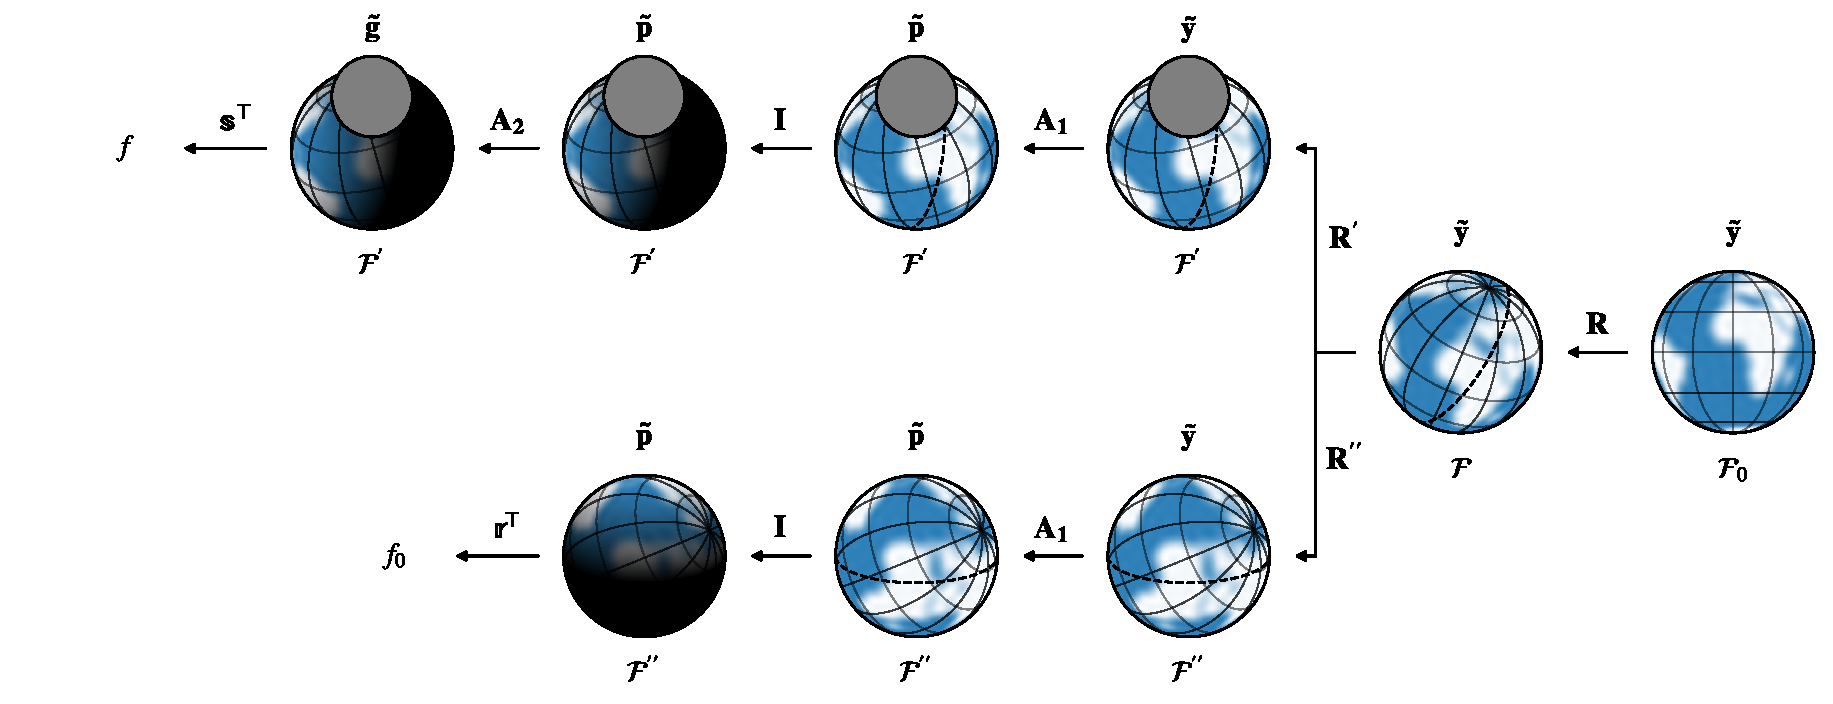
\includegraphics[width=\linewidth]{figures/frames.pdf}
        \oscaption{frames}{%
            How \starry computes the flux from a body in reflected light,
            tracking each of the linear transformations from the input map
            (far right) to the output (far left). The label below each map
            denotes the reference frame, while the label above
            each map denotes the basis in which the map is represented.
            Arrows indicate linear operations and are labeled accordingly.
            The upper branch corresponds to the occulted case
            (Equation~\ref{eq:sTA2IA1RRy}), while the
            lower branch corresponds to the case where the body
            is unocculted (Equation~\ref{eq:rTIA1RRy}).
            See text for details.
            \label{fig:frames}
        }
    \end{centering}
\end{figure}

We may now re-write Equations~(\ref{eq:sTARRy}) and (\ref{eq:rTA1Ry}) to
account for this illumination transformation. The flux during an occultation
is now given by
%
\begin{align}
    \label{eq:sTA2IA1RRy}
    f & =
    \mathfrak{s}^\top(b, \theta', b_o, r_o)
    \BF{A_2}
    \BF{I}(b, \theta', r_s)
    \BF{A_1}
    \BF{R}'(x_o, y_o)
    \BF{R}(i, \lambda, \vartheta)
    \BF{y}
    \quad,
\end{align}
%
where
%
\begin{align}
    \label{eq:theta'}
    \theta' = \mathrm{arctan2}(x_o, y_o) - \mathrm{arctan2}(x_s, y_s)
\end{align}
%
is the angle of the terminator in the frame $\mathcal{F}'$.
Note that we made use of the fact that
$\BF{A} = \BF{A_2} \BF{A_1}$
(Equation~\ref{eq:A}), where $\BF{A_1}$ transforms from
the spherical harmonic basis $\by$ to the polynomial basis $\bp$, and
$\BF{A_2}$ transforms from $\bp$ to the Green's basis $\bg$.

Similarly, the flux when there is no occultation is now given by
%
\begin{align}
    \label{eq:rTIA1RRy}
    f_0 & =
    \mathfrak{r}^\top(b)
    \BF{I}(b, \theta'', r_s)
    \BF{A_1}
    \BF{R}''(x_s, y_s)
    \BF{R}(i, \lambda, \vartheta)
    \BF{y}
    \quad,
\end{align}
%
where
%
\begin{align}
    \label{eq:theta''}
    \theta'' = 0
\end{align}
%
is the angle of the terminator in the frame $\mathcal{F}''$, by
construction. The transformation
$\BF{R}'' = \BF{R}''(x_s, y_s)$ (Equation~\ref{eq:R''}) rotates
the body so the semi-major axis of the terminator is aligned
with the $x''$-axis; as will become clear in \S\ref{sec:solution-no-occ} below,
this greatly simplifies the integration step.

Note that in both equations we replaced the integral vectors
$\rTe$ and $\sTe(b_o, r_o)$
with the vectors
$\mathfrak{r}^\top(b)$ and $\mathfrak{s}^\top(b, \theta', b_o, r_o)$,
respectively.
As we mentioned above, we must modify the integration limits to exclude the
nightside, where the weighting by $\BF{I}$ is unphysical.
The vectors $\mathfrak{r}^\top$ and $\mathfrak{s}^\top$ correspond to these
modified integrals, which we devote the rest of this paper to
computing.

Figure~\ref{fig:frames} summarizes the transformations involved in the two
equations above. Starting on the right with a map vector $\BF{y}$ in
the spherical harmonic basis $\by$, defined in some observer-independent frame
$\mathcal{F}_0$, we first rotate it via $\BF{R}$ to the sky frame
$\mathcal{F}$, in which the body is viewed by the
observer. If an occultor is present (upper branch of the figure),
we rotate the map from $\mathcal{F}$ via $\BF{R}'$ to the frame
$\mathcal{F}'$, in which the occultor lies along the
$+y'$-axis. We then apply $\BF{A_1}$ to change basis to $\bp$ and $\BF{I}$
to weight the map by the illumination. Finally, we change basis
via $\BF{A_2}$ to the Green's basis, in which we compute and dot the
integrals $\sT$.
If, on the other hand, there is no occultation (lower branch of the figure),
we instead rotate the map via $\BF{R}''$ to the integration frame
$\mathcal{F}''$, in which the terminator is parallel to the
$x''$-axis. We then apply $\BF{A_1}$ to change basis to $\bp$, apply the
illumination transform $\BF{I}$, and finally dot in the solutions to the
surface integrals $\rT$.

%

\section{The Solution: No Occultation}
\label{sec:solution-no-occ}
%
Before we tackle configurations involving occultations, we must address the
simpler problem of computing the total visible flux from an unocculted
body in reflected light (Equation~\ref{eq:rTIA1RRy}). This problem was
originally solved by \citet{Haggard2018} and subsequently by
\citet{Luger2019b}, but for completeness we present the detailed
derivation in the \starry formalism here.

As we discussed above, we perform the integration in a frame
$\mathcal{F}''$
in which the semi-major axis of the terminator is aligned with the
$x''$-axis, with the illumination source at $y'' \ge 0$.
The solution vector may then be computed from
%
\begin{align}
    \label{eq:rT}
    \rT(b) & =
    \int_{-1}^{1}
    \int_{b\sqrt{1 - x''^2}}^{\sqrt{1 - x''^2}}
    \bp(x'', y'')
    \ \dd y'' \ \dd x''
    \quad,
\end{align}
%
which is identical to Equation~(20) in \citet{Luger2019} except for the
lower integration limit of the inner integral. The lower limit is now
the equation describing the terminator, which ensures we always exclude the
nightside from the integration region.
%
For computational efficiency, in practice we compute the integral of the
intensity-weighted basis directly,
%
\begin{align}
    \label{eq:rTI}
    \BS{\rho}^\top(b, r_s) & \equiv
    \rT(b) \mathbf{I}(b, 0, r_s)
    \nonumber                       \\
                           & =
    \int_{-1}^{1}
    \int_{b\sqrt{1 - x''^2}}^{\sqrt{1 - x''^2}}
    \bp(x'', y'')
    \mathbf{I}(b, 0, r_s)
    \ \dd y'' \ \dd x''
    \quad,
\end{align}
%
recalling that in frame $\mathcal{F}''$, $\theta'' = 0$ by
definition.
%
Equation~(\ref{eq:rTI}) may be solved analytically in terms of purely
trigonometric and algebraic functions of $b$. The component of $\BS{\rho}^\top$
at index $n$ is given by
%
\begin{proof}{}
    \label{eq:rTsoln}
    \rho_n(b, r_s) & =
    \frac{1}{4\pi r_s^2}
    \begin{cases}
        \frac{b_c\left(1 - b^{\frac{\nu + 4}{2}}\right)}{2}
        J_{\frac{\mu}{2}, \frac{\nu + 2}{2}} -
        b H_\frac{\nu}{2}(b) K_{\frac{\mu}{2}, \frac{\nu}{2}}
        %
         &
        %
        \qquad
        \mu, \nu \ \mathrm{even}
        %
        \\[1em]
        %
        b_c
        H_{\frac{\nu + 1}{2}}(b) K_{\frac{\mu - 1}{2}, \frac{\nu + 1}{2}}
        %
        \\[0.5em]
        \qquad
        %
        - \frac{b}{2} \bigg\{
        \left(1 - b^{\frac{\nu + 1}{2}}\right)
        \left(
        J_{\frac{\mu - 1}{2}, \frac{\nu - 1}{2}} -
        J_{\frac{\mu + 3}{2}, \frac{\nu - 1}{2}}
        \right)
        \\[0.5em]
        \qquad\qquad
        -
        \left(1 - b^{\frac{\nu + 5}{2}}\right)
        J_{\frac{\mu - 1}{2}, \frac{\nu + 3}{2}}
        \bigg\}
        %
         &
        %
        \qquad
        \mathrm{otherwise}
        %
    \end{cases}
\end{proof}
%
where we make use of the indices
%
\begin{align}
    \label{eq:l-m-mu-nu}
    \mu & = l - m
    \nonumber                 \\
    \nu & = l + m
    \nonumber                 \\
    l   & = \floor*{\sqrt{n}}
    \nonumber                 \\
    m   & = n - l^2 - l
\end{align}
%
as in \citet{Luger2019} and we define the helper functions
%
\begin{proof}{}
    \label{eq:HJK}
    H_{j}(b) &= \int_b^1 a^j \sqrt{1 - a^2} \dd a
    \nonumber \\
    %
    J_{i,j} &=
    \frac{
        \Gamma\left(\frac{i + 1}{2}\right)
        \Gamma\left(\frac{j + 1}{2}\right)
    }
    {
        \Gamma\left(\frac{i + j + 4}{2}\right)
    }
    %
    \nonumber \\
    %
    K_{i,j} &=
    \frac{
        \Gamma\left(\frac{i + 1}{2}\right)
        \Gamma\left(\frac{j + 4}{2}\right)
    }
    {
        \Gamma\left(\frac{i + j + 5}{2}\right)
    }
    \quad.
\end{proof}
%
Given initial conditions
%
\\[1em]
\begin{minipage}{.33\linewidth}
    \begin{align}
        H_{0}(b) & = \frac{\arccos(b) - bb_c}{2}
        %
        \nonumber                                \\
        %
        H_{1}(b) & = \frac{b_c^3}{3}
        %
        \nonumber
    \end{align}
\end{minipage}%
\begin{minipage}{.32\linewidth}
    \begin{align}
        J_{0,0} & = \pi
        %
        \nonumber               \\
        %
        J_{0,1} & = \frac{4}{3}
        %
        \nonumber
    \end{align}
\end{minipage}%
\begin{minipage}{.33\linewidth}
    \begin{proof}{}
        \label{eq:IJK0}
        K_{0,0} &= \frac{4}{3}
        %
        \nonumber \\
        K_{0,1} &= \frac{3\pi}{8}
    \end{proof}
\end{minipage}
\\[1em]
%
we may compute all higher order terms from the recurrence relations
%
\begin{proof}{}
    \label{eq:IJKrec}
    H_{j}(b) &= \frac{b^n b_c^3 + (j - 1) H_{j - 2}(b)}{j + 2}
    %
    \nonumber \\
    %
    J_{0,j} &= \left(\frac{j - 1}{j + 2}\right) J_{0,j-2}
    %
    \nonumber \\
    %
    K_{0,j} &= \left(\frac{j + 2}{j + 3}\right) K_{0,j-2}
    %
    \nonumber \\
    %
    J_{i,j} &= \left(\frac{i - 1}{i + j + 2}\right) J_{i-2,j}
    %
    \nonumber \\
    %
    K_{i,j} &= \left(\frac{i - 1}{i + j + 3}\right) K_{i-2,j}
    \quad.
\end{proof}
%
Once $\BS{\rho}^\top$ is known, the observed flux is computed from
(c.f. Equation~\ref{eq:rTIA1RRy})
%
\begin{proof}{}
    \label{eq:f0}
    f_0 & =
    \BS{\rho}^\top(b, r_s)
    \BF{A_1}
    \BF{R}''(x_s, y_s)
    \BF{R}(i, \lambda, \vartheta)
    \BF{y}
    \quad.
\end{proof}
%
Finally, for future reference, we can also compute what we will call the
\emph{complement} of case 0:
%
\begin{proof}{}
    \label{eq:f0hat}
    \hat{f}_0 & =
    -\BS{\rho}^\top(-b, r_s)
    \BF{A_1}
    \BF{R}''(-x_s, -y_s)
    \BF{R}(i, \lambda, \vartheta)
    \BF{y}
    \quad,
\end{proof}
%
This is the flux we would get if we placed a \emph{negative} illumination
source at the antipode $(-x_s, -y_s, -z_s)$ of the true source, and
will be useful in negating the unphysical negative contribution from our
polynomial illumination function (Equation~\ref{eq:illum_poly}) in
the following section.

\section{The Solution: Occultation}
\label{sec:solution-occ}
%
The integration in the unocculted case presented above is relatively
straightforward, since
the boundaries of integration are always the half-ellipse defining the
terminator and the half-circle defining the upper limb of the body
(Equation~\ref{eq:rT}). When an occultor is present, however, the
integration boundaries are far less trivial, since they may or may not
include sections of the terminator, sections of the limb of the body,
and sections of the limb of the occultor. There are in total 14 families of
configurations, each defined by a distinct combination of integration
boundaries; these are shown in Figures~\ref{fig:cases} and
\ref{fig:pathological}.
Together, these cases encompass all possible
occultation configurations, for any illumination angle, occultor size, and
occultor position.

\xxx{In general, we do not just integrate over the dayside.}

Before we discuss how to compute the occultation integrals, we must first
develop a procedure to identify the relevant case given the occultor
impact parameter $b_o = \sqrt{x_o^2 + y_o^2}$ and radius $r_o$ and
the terminator semi-minor
axis $b$ and angle $\theta'$ in the frame $\mathcal{F}'$.
Then, once the case is determined, we must
identify the relevant integration boundaries, which depend on the points
of intesection between the limb of the body, the limb of the occultor, and
the terminator. We do so in the following sections.

%

\subsection{Case determination}
\label{sec:which-case}

\begin{figure}[t!]
    \begin{centering}
        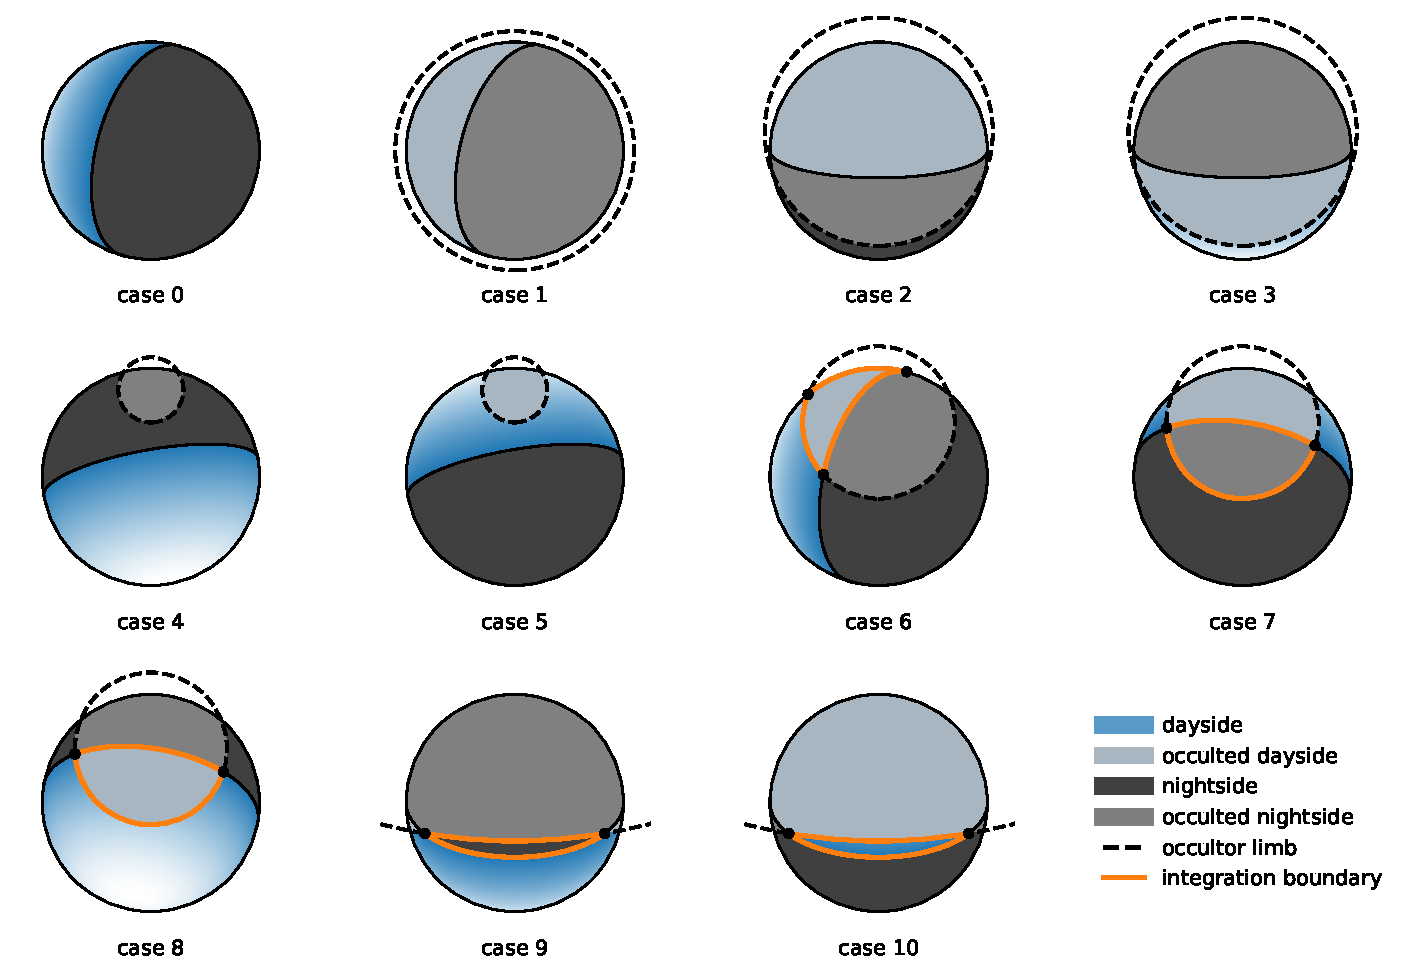
\includegraphics[width=\linewidth]{figures/cases.pdf}
        \oscaption{cases}{%
            The 10 principal families of cases of occultations in
            reflected light.
            In these figures, the body with the solid outline
            is the one whose flux we are interested in, and the body with the
            dashed outline is the occultor.
            The nightside of the occulted body is colored
            black (dark grey if occulted), and the dayside is colored blue
            (bluish-grey if occulted).
            Case 0 is the unocculted case (\S\ref{sec:solution-no-occ}),
            while cases 1--5 involve
            configurations in which the limb of the occultor does not intersect
            with the terminator at any point, so the visible flux may be
            computed in terms of classical \starry integrals. The remaining
            cases require integration along the orange boundary (the curves
            $P$, $T$, and $Q$ of
            \S\ref{sec:cases-hard}), which
            include the terminator. These involve the evaluation of incomplete
            elliptic integrals and are derived below.
            \label{fig:cases}
        }
    \end{centering}
\end{figure}

The key to identifying the case corresponding to a given configuration is
to determine whether or not the limb of the occultor intersects the terminator
of the body, and if so, the points of intersection.
While we perform the integration in frame $\mathcal{F}'$, finding the points
of intersection with the terminator is easier if we temporarily switch to
the frame $\mathcal{F}''$ (via Equation~\ref{eq:R''}) in which the terminator
is parallel to the $x''$-axis.
In this frame, the equations defining the terminator and the limb of the
occultor are, respectively,
%
\begin{proof}{}
    y''_1(x'') & = b \sqrt{1 - x''^2}
    \nonumber                                               \\
    y''_2(x'') & = y''_o \pm \sqrt{r_o^2 - (x'' - x''_o)^2}
\end{proof}
%
where
%
\begin{proof}{}
    x''_o = b_o\sin\theta'
    \nonumber \\
    y''_o = b_o\cos\theta'
\end{proof}
%
are the coordinates of the occultor in $\mathcal{F}''$.
%
We wish to find the set of $N$ points
$\BS{x''} = \{x_n''~\big|~0~\le~n~<~N\}$
for which
$y''_1(x_n'') - y''_2(x_n'') = 0$. Following \citet{Luger2017}, we may
express this condition as the quartic equation
%
\begin{proof}{}
    \label{eq:quartic}
    A {x''}^4 + B {x''}^3 + C {x''}^2 + D {x''} + E = 0
\end{proof}
%
with coefficients
%
\begin{proof}{}
    \label{eq:quartic-coeffs}
    A &= (1 - b^2)^2
    \nonumber \\
    B &= -4 x''_o (1 - b^2)
    \nonumber \\
    C &= -2 \bigg(
    b^4
    + r_o^2
    - 3 {x''_o}^2
    - {y''_o}^2
    - b^2 \big(1 + r_o^2 - {x''_o}^2 + {y''_o}^2\big)
    \bigg)
    \nonumber \\
    D &= -4 x''_o (b^2 - r_o^2 + {x''_o}^2 + {y''_o}^2)
    \nonumber \\
    E &=
    b^4
    - 2 b^2 \big(r_o^2 - {x''_o}^2 + {y''_o}^2\big)
    + \big(r_o^2 - {x''_o}^2 - {y''_o}^2\big)^2
    \quad.
\end{proof}
%
Although closed-form solutions to quartic equations exist
\citep[see, e.g.,][who solve for the area of overlap between two ellipses
    analytically]{Hughes2011}, they are prone to significant numerical
instabilities. Instead, we solve for the roots of the quartic
numerically by casting it
as an eigenvalue problem \citep[e.g.,][]{Edelman1995} and polish the
results with a few iterations of Newton's method. We find that this is
reasonably computationally efficient and
yields roots with precision within a couple orders of magnitude of machine
epsilon (see \S\ref{sec:performance}).

In general, the quartic defined by Equation~(\ref{eq:quartic}) has
$N=4$ (potentially degenerate) roots, some of which may be complex, and some
of which correspond to intersections with the wrong half of the
terminator ellipse (i.e., the section of the terminator on the far side
of the body). After excluding the unphysical solutions, we are still left with
anywhere between zero and four roots.

Cases with zero roots (case 1 -- case 4) are treated in \S\ref{sec:cases-easy},
while cases with one or two roots (case 5 -- case 8) are treated in
\S\ref{sec:cases-hard}. Cases with three or four roots
(case 9 -- case 10) are rarely encountered
in practice, but are possible for some pathological configurations; these are
treated in \S\ref{sec:cases-pathological}.

%

\subsection{Cases 1--5}
\label{sec:cases-easy}
%
Cases 1--5 (see Figure~\ref{fig:cases}) involve configurations in which the
occultor does not intersect with
the terminator of the occulted body, and are therefore fairly
straightforward to solve. In particular, we can use the original emitted
light solution from \citet{Luger2019}, provided we weight the map by our
polynomial illumination function:
%
\begin{proof}{}
    \label{eq:fI}
    f_I &=
    \sTe(b_o, r_o)
    \BF{A_2}
    \BF{I}(b, \theta', r_s)
    \BF{A_1}
    \BF{R}'(x_o, y_o)
    \BF{R}(i, \lambda, \vartheta)
    \BF{y}
    \quad,
\end{proof}
%
where $\sTe(b_o, r_o)$ is the emitted light solution vector
\citep[Equation~26 in][]{Luger2019}. The flux $f_I$ is the flux one would
measure from a body whose surface map is weighted by the illumination function
$\BF{I}(b, \theta', r_s)$ during an occultation. Note that this is not
necessarily the \emph{observed} flux, since this may include the unphysical
negative contribution from the nightside. We must compute the actual
observed flux on a case-by-case basis.

Case 1 corresponds to any complete occultation of the body
($b_o \le r_o - 1$), so the solution for the flux is trivial:
%
\begin{align}
    \label{eq:f1}
    f_1 = 0
    \quad.
\end{align}
%
Case 2 corresponds to occultations in which the occultor blocks \emph{all} of
the dayside of the body and \emph{some} of the nightside. In this
configuration, the unocculted part of the disk consists only of nightside, so
the solution is again trivial:
%
\begin{align}{}
    \label{eq:f2}
    f_2 = 0
    \quad.
\end{align}
%
Conversely, case 3 corresponds to occultations in which the occultor blocks
\emph{all} of the nightside of the body and \emph{some} of the dayside.
Since the visible portion of the disk consistss only of dayside, we can
simply use the weighted solution in emitted light
(Equation~\ref{eq:fI}):
%
\begin{proof}{}
    \label{eq:f3}
    f_3 = f_\mathrm{I}
\end{proof}
%
Case 4 involves any occultation in which the occultor blocks \emph{only} the
nightside of the body (regardless of whether or not it intersects with the
limb of the body). Since the nightside intensity is zero everywhere, this case
is also trivial, as the flux is equal to the flux in the no occultation case
(Equation~\ref{eq:f0}):
%
\begin{align}
    \label{eq:f4}
    f_2 = f_0
    \quad.
\end{align}
%
Finally, case 5 involves any occultation in which the occultor blocks
\emph{only} the dayside of the body (regardless of whether or not it
intersects with the limb). We first compute the illumination-weighted flux
$f_I$ as above, then negate the unphysical nightside contribution
using Equation~(\ref{eq:f0hat}):
%
\begin{proof}{}
    \label{eq:f5}
    f_5 = f_I - \hat{f}_0
    \quad.
\end{proof}

%

\subsection{Cases 6--10}
\label{sec:cases-hard}
%

\begin{figure}[t!]
    \begin{centering}
        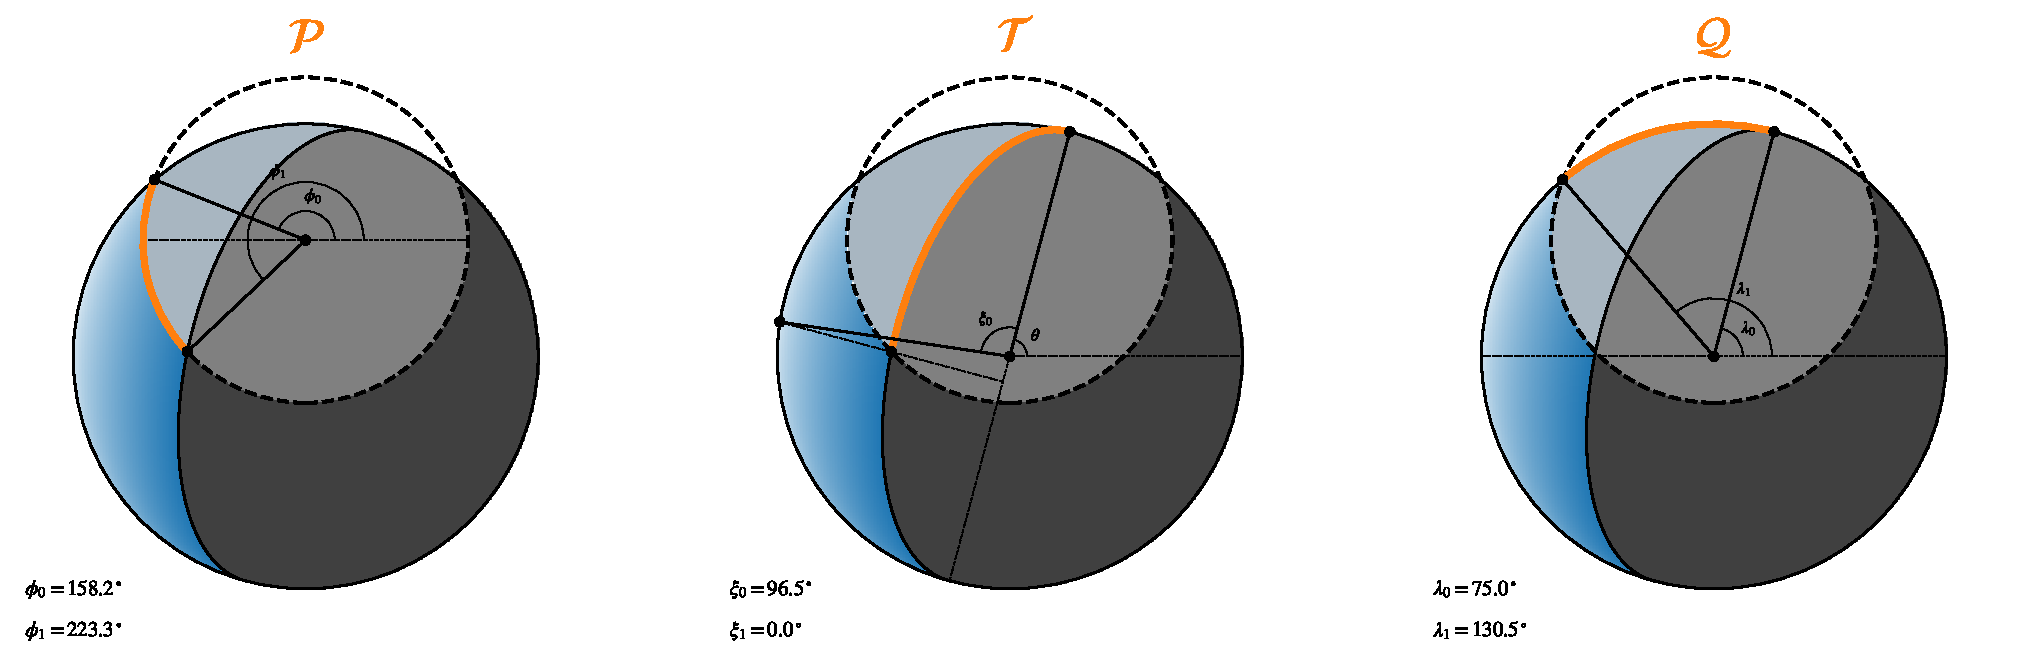
\includegraphics[width=\linewidth]{figures/geometry.pdf}
        \oscaption{geometry}{%
            Geometry of an occultation in reflected light, corresponding
            to case 6 in Figure~\ref{fig:cases}. The surface integral over
            the occulted portion of the dayside (bluish-grey region)
            is computed from the line integrals of the antiderivatives of the
            surface intensity map along the boundary curves
            $P$, $T$, and $Q$. See text for details.
            \label{fig:geometry}
        }
    \end{centering}
\end{figure}

Cases 6--10 (see Figure~\ref{fig:cases}) correspond to configurations in which
the limb of the occultor intersects with the terminator at either one point
(case 6) or two points (cases 7--10). Because of these intersections, we
cannot simply re-weight the emitted light solution, as the integration
boundaries are now different. In general, we may compute the flux by
integrating the components of the Green's basis $\bg$
over the region $S$ bounded by three curves, which we denote
$P$, $T$, and $Q$. These are shown in orange
in Figure~\ref{fig:cases} and presented in more detail in
Figure~\ref{fig:geometry}.
Curve $P$ is a segment of the limb of
the occultor, parametrized by the angle $\phi \in [\phi_0, \phi_1]$;
curve $T$ is a segment of the terminator,
parametrized by the angle $\xi \in [\xi_0, \xi_1]$;
and curve $Q$ is a segment of the limb of the occulted body,
parametrized by the angle $\lambda \in [\lambda_0, \lambda_1]$.
The endpoints $\phi_0, \phi_1, \xi_0, \xi_1, \lambda_0,$ and
$\lambda_1$ are functions of the solutions to the quartic from
\S\ref{sec:which-case} and will be presented in \S\ref{sec:sT}.

Let $\sT$ be the integral of $\bg^\top$ over $S$:
%
\begin{align}
    \label{eq:sTint}
    \sT(b, \theta', b_o, r_o) & =
    \iint\limits_{S(b, \theta', b_o, r_o)}
    \bg^\top(x', y')
    \ \dd x' \ \dd y'
    \quad,
\end{align}
%
We defer the solution to Equation~(\ref{eq:sTint}) to \S\ref{sec:sT} below,
as it is quite lengthy. Given $\sT$, the flux $f_S$ over the integration
region $S$ is computed from Equation~(\ref{eq:sTA2IA1RRy}):
%
\begin{align}
    \label{eq:fS}
    f_S & =
    \mathfrak{s}^\top(b, \theta', b_o, r_o)
    \BF{A_2}
    \BF{I}(b, \theta', r_s)
    \BF{A_1}
    \BF{R}'(x_o, y_o)
    \BF{R}(i, \lambda, \vartheta)
    \BF{y}
    \quad.
\end{align}
%
Note again that this is not necessarily the \emph{observed} flux, which we must
compute on a case-by-case basis below.

Case 6 corresponds to configurations in which the limb of the occultor
intersects the terminator at a single point. The integration region
(see Figures~\ref{fig:cases} and \ref{fig:geometry}) is the occulted
portion of the dayside, which is bounded by all three curves $P$, $Q$, and $T$.
The total flux may
be computed by subtracting the occulted flux $f_S$ from the total dayside
flux $f_0$:
%
\begin{proof}{}
    \label{eq:f6}
    f_6 = f_0 - f_S
    \quad.
\end{proof}
%
Cases 7--10 involve two points of intersection between the occultor limb and
the terminator.
%
Cases 7 and 8 correspond to occultors that block some of the
nightside and some of the dayside, but \emph{neither} of the extrema of the
terminator ellipse. In case 7 a lens-shaped region is formed by the
intersection of the occultor limb and the terminator on the
\emph{nightside}, while in case 8 this region is formed on the \emph{dayside}.
%
In case 7, we begin by computing the
flux over the unocculted region, $f_I$, which includes the spurious
nightside contribution. We then remove this contribution by noting that it
is equal to the total nightside contribution, $\hat{f}_0$, minus the
occulted nightside flux, $f_S$:
%
\begin{proof}{}
    \label{eq:f7}
    f_7 = f_I - (\hat{f}_0 - f_S)
    \quad.
\end{proof}
%
Case 8, on the other hand, is topologically equivalent to case 6, since
the integration region consists of occulted dayside:
%
\begin{proof}{}
    \label{eq:f8}
    f_8 = f_0 - f_S
    \quad.
\end{proof}
%
Cases 9 and 10 correspond to occultors that also block some nightside and some
dayside, along with \emph{both} of the extrema of the ellipse; these are
therefore exclusively for large occultors ($r_o > 1$). Case 9
involves occultations in which only a small lens-shaped region of the
nightside is visible. The total flux is the visible dayside plus unphysical
nightside contribution, $f_I$, minus the nightside contribution, which we
compute from Equation~(\ref{eq:fS}):
%
\begin{proof}{}
    \label{eq:f9}
    f_9 = f_I - f_S
    \quad.
\end{proof}
%
Conversely, case 10 involves occultations in which only a small lens-shaped
region of the dayside is visible. In this case, we may compute the observed
flux from Equation~(\ref{eq:fS}) directly:
%
\begin{proof}{}
    \label{eq:f10}
    f_{10} = f_S
    \quad.
\end{proof}
%

\subsection{Cases 11--14}
\label{sec:cases-pathological}

\begin{figure}[t!]
    \begin{centering}
        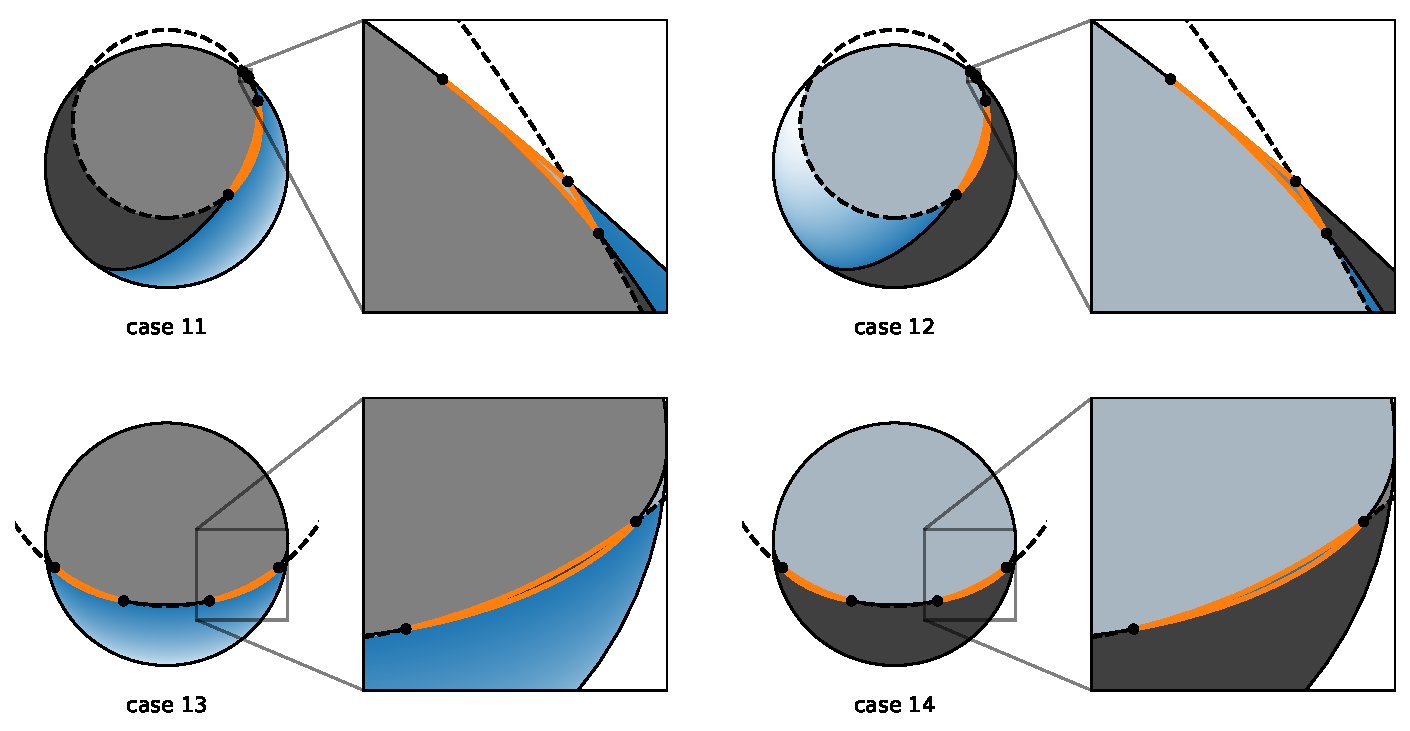
\includegraphics[width=\linewidth]{figures/pathological.pdf}
        \oscaption{pathological}{%
            Four additional families of occultations in reflected light,
            involving rare triple (cases 11 and 12, top) and quadruple
            (cases 13 and 14, bottom) intersections between the limb of the
            occultor and the terminator of the occulted body. All four cases
            involve integration over two disjoint regions (bounded by
            the orange curves in the figure). The insets next to each case
            show a zoomed-in version of four such regions. See text for
            more details.
            \label{fig:pathological}
        }
    \end{centering}
\end{figure}

Cases 11--14 correspond to (rare) configurations involving three
or four roots to Equation~\ref{eq:quartic} and are
illustrated in Figure~\ref{fig:pathological}. All four involve integration over
two disjoint regions (see the figure).
%
Cases 11 and 12 involve three points of intersection between the terminator
and the occultor limb. In case 11, the regions of integration $S_1$ and
$S_2$ are the
occulted portion of the dayside, so the solution is similar to
that of cases 6 and 8:
%
\begin{proof}{}
    \label{eq:f11}
    f_{11} = f_0 - (f_{S_1} + f_{S_2})
    \quad,
\end{proof}
%
where $f_{S_1}$ and $f_{S_2}$ are computed from Equation~(\ref{eq:fS}) for
each of the integration regions. Conversely, in case 12 the two regions
are the occulted portion of the nightside, so the solution is similar to that
of case 7:
%
\begin{proof}{}
    \label{eq:f12}
    f_{12} = f_I - \big(\hat{f}_0 - (f_{S_1} + f_{S_2})\big)
    \quad,
\end{proof}
%
Finally, cases 13 and 14 involve four points of intersection between the
terminator and the occultor limb. The regions of integration in case 13 are
the visible portion of the nightside, so this case is equivalent to case 9:
%
\begin{proof}{}
    \label{eq:f13}
    f_{13} = f_I - (f_{S_1} + f_{S_2})
    \quad.
\end{proof}
%
Conversely, the regions of integration in case 14 are the
visible portion of the dayside, so this case is equivalent to case 10:
%
\begin{proof}{}
    \label{eq:f14}
    f_{14} = f_{S_1} + f_{S_2}
    \quad.
\end{proof}
%

\subsection{Computing the integrals $\sT$}
\label{sec:sT}
%
In the previous sections, we discussed how to identify the case
corresponding to a specific configuration of the occultor and the
illumination source. We showed how in some cases
(1--5; \S\ref{sec:cases-easy}) the total flux may be
computed by exploiting the classical \starry integrals (Equation~\ref{eq:fI}).
In all other cases (6--14; \S\ref{sec:cases-hard} and
\S\ref{sec:cases-pathological}), however, the flux computation involves
evaluation of
Equation~(\ref{eq:fS}), where the solution vector $\mathfrak{s}^\top$
is the vector of integrals (in the frame $\mathcal{F}'$)
of each of the terms in the Green's basis $\bg$
over a region $S$ of the
projected disk of the occultor (Equation~\ref{eq:sTint}).
%
As in \citet{Luger2019}, the approach to computing $\sT$
is to use Green's theorem to transform the surface integrals into line
integrals along the curves $P$, $T$, and $Q$
(see Figure~\ref{fig:geometry}). Specifically, we write%
\footnote{%
    In this section, we deliberately drop the dependence of $\sT$ and
    the primitive
    integrals on the geometrical parameters $b, \theta', b_o, r_o$
    for clarity.
}
%
\begin{align}
    \label{eq:greens}
    \sT
     & =
    \iint\limits_{S}
    \bg^\top(x', y')
    \ \dd x' \ \dd y'
    \nonumber \\[0.5em]
     & =
    \oint \bvec{G}^\top (x', y') \cdot
    \dd \bvec{r} (x', y')
    \quad,
\end{align}
%
where $\bvec{G} (x', y')$
is an array of two-dimensional Cartesian vectors chosen such that its
exterior derivative is $\bg$,
%
\begin{align}
    \label{eq:DGg}
    \frac{\dd \bvec{G}_{y'}(x', y')}{\dd x'}
    - \frac{\dd \bvec{G}_{x'}(x', y')}{\dd y'} = \bg(x', y')
    \quad,
\end{align}
%
and
%
\begin{align}
    \dd \BF{r} (x', y') & =
    \left(\frac{\dd x'}{\dd \varphi}\right) \dd \varphi \, \xhat' +
    \left(\frac{\dd y'}{\dd \varphi}\right) \dd \varphi \, \yhat'
    \quad,
\end{align}
%
where $\varphi$ is the parametrized angle along the integration path
and the integral is taken in a counter-clockwise direction relative to
the center of the integration region.
%
\citet{Luger2019} showed that one possible solution to
Equation~(\ref{eq:DGg}) consists of the vector whose $n^\mathrm{th}$
component is given by
%
\begin{align}
    \label{eq:G}
    \BF{G}_n (x, y) & =
    \begin{dcases}
        %
        x'^{\frac{\mu + 2}{2}}
        y'^{\frac{\nu}{2}}
        \,\yhat'
         & \qquad \mu, \nu \, \mathrm{even}
        \\[1em]
        %
        \frac{1-z(x', y')^3}{3(1-z(x', y')^2)}\bigg(-y' \, \xhat' + x' \, \yhat'\bigg)
         & \qquad \mu = \nu = 1
        \\[1em]
        %
        x'^{l-2}
        z(x', y')^3
        \,\xhat
         & \qquad \nu \, \mathrm{odd}, \,
        \mu = 1, \,
        l \, \mathrm{even}
        \\[1em]
        %
        x'^{l-3}
        y'
        z(x', y')^3
        \,\xhat
         & \qquad \nu \, \mathrm{odd}, \,
        \mu = 1, \,
        l \, \mathrm{odd}
        \\[1em]
        %
        x'^{\frac{\mu-3}{2}}
        y'^{\frac{\nu-1}{2}}
        z(x', y')^3
        \,\yhat
         & \qquad \mathrm{otherwise,}
    \end{dcases}
\end{align}
%
where the indices $l, m, \mu, \nu$ are given by Equation~(\ref{eq:l-m-mu-nu}).

We showed in the previous sections that there are at most three curves
$P$, $T$, and $Q$ bounding a given closed surface of integration
(see Figure~\ref{fig:geometry}). We may therefore express
Equation~(\ref{eq:greens}) as
%
\begin{proof}{}
    \label{eq:sT}
    \sT & =
    \mathfrak{p}^\top + \mathfrak{t}^\top + \mathfrak{q}^\top
    \quad,
\end{proof}
%
where we define the primitive integrals%
\footnote{%
    The components of the vectors $\mathfrak{p}^\top$ and
    $\mathfrak{q}^\top$ are analogous to the primitive integrals
    $\mathcal{P}$ and $\mathcal{Q}$
    defined in Equations~(30)--(32) in \citet{Luger2019}, although the
    integration limits of both and the sense of integration of $\mathcal{P}$
    are different.
}
%
\begin{proof}{}
    \label{eq:pT}
    \mathfrak{p}^\top
    & =
    \int\limits_{\BS{\phi}}
    \mathbf{G}^\top(x'_p, y'_p)
    \cdot \dd \mathbf{r}(x'_p, y'_p)
    %
    \\
    %
    \label{eq:tT}
    \mathfrak{t}^\top
    & =
    \int\limits_{\BS{\xi}}
    \mathbf{G}^\top(x'_t, y'_t)
    \cdot \dd \mathbf{r}(x'_t, y'_t)
    %
    \\
    %
    \label{eq:qT}
    \mathfrak{q}^\top
    & =
    \int\limits_{\BS{\lambda}}
    \mathbf{G}^\top(x'_q, y'_q)
    \cdot \dd \mathbf{r}(x'_q, y'_q)
\end{proof}
%
to be the line integrals of $\mathbf{G}$ along each of the curves
$P$, $T$, and $Q$, respectively, where the coordinates along each
curve are parametrized
in terms of $\varphi$ as follows:
%
\\[1em]
%
\begin{minipage}{0.31\linewidth}
    \begin{align}
        x'_p & = r_o \cos\varphi
        \nonumber                      \\
        y'_p & = b_o + r_o \sin\varphi
        \nonumber
    \end{align}
\end{minipage}
%
\begin{minipage}{0.35\linewidth}
    \begin{align}
        x'_t & = \cos\theta' \cos\varphi - b \sin\theta' \sin\varphi
        \nonumber                                                    \\
        y'_t & = \sin\theta' \cos\varphi + b \cos\theta' \sin\varphi
        \nonumber
    \end{align}
\end{minipage}
%
\begin{minipage}{0.31\linewidth}
    \begin{proof}{}
        \label{eq:xy_pqt}
        x'_q & =\cos\varphi
        \nonumber           \\
        y'_q & = \sin\varphi
        \quad,
    \end{proof}
\end{minipage}
%
\\[1em]
%
and we define
%
\begin{align}
    \int\limits_{\BS{\varphi}} & \equiv
    %
    \int\limits_{\varphi_{0}}^{\varphi_{1}}
    +
    \int\limits_{\varphi_{2}}^{\varphi_{3}}
    +
    \cdots
    +
    \int\limits_{\varphi_{N - 2}}^{\varphi_{N - 1}}
    %
    \nonumber                           \\
                               & \equiv
    \sum_{i = 0}^{\frac{N - 1}{2}}
    \int\limits_{\varphi_{2i}}^{\varphi_{2i+1}}
\end{align}
%
to be the sum of definite integrals between pairs of limits $\varphi_i$
arranged in an array $\BS{\varphi}$ of length $N$.
For cases involving integration over a single closed region, this
corresponds to a single integral. For cases 11--14, this corresponds to
the sum of two integrals, one for each of the two disjoint regions.
In the next three sections, we derive the solutions to each of these
primitive integrals.

\subsection{The integral along the occultor limb, $\mathfrak{p}^\top$}
\label{sec:pT}
%
In this section we present a solution to Equation~(\ref{eq:pT}). The first
order of business is to derive expressions for the integration limits
$\BS{\phi}$. Depending on the integration case, these limits will correspond
to the point of intersection between the limb of the occultor and the
limb of the occulted body and/or the point of intersection between the limb
of the occultor and the terminator of the occulted body.
The former is given by
\citep[c.f. Equation~24 in][]{Luger2019}
%
\begin{align}
    \phi_l & = \frac{\pi}{2} \pm \left(\arcsin\left(\frac{1 - r_o ^ 2 - b_o ^ 2}{2 b_o r_o}\right) - \frac{\pi}{2}\right)
    \quad,
\end{align}
%
where the sign is chosen such that the point
$(r_o\cos\phi_l, b_o + r_o\sin\phi_l)$ is on the dayside of the occulted body,
and the latter (of which there may be multiple) is given by
%
% Introduce the function
% %
% \begin{proof}{}
%     \textrm{\faAdjust}(x, y) &=
%     \begin{cases}
%         \textrm{\faCircleO} & \qquad -x \sin\theta' + y\cos\theta' \ge b \sqrt{1 - (x\cos\theta' + y\sin\theta') ^ 2}
%         \\
%         \textrm{\faCircle}  & \qquad \mathrm{otherwise}
%     \end{cases}
% \end{proof}
% %
% which returns \faCircleO\ if point $(x, y)$ is on the dayside of the body and
% \faCircle\ if it is on the nightside.
%
%
\begin{align}
    \BS{\phi_t} & =
    \theta' + \mathrm{arctan2}\left(b\sqrt{1 - \BS{x''}^2 - y''_o}, \BS{x''} - x''_o\right)
    \quad
\end{align}
%
where $\BS{x''}$ are the roots of the quartic (Equation~\ref{eq:quartic}).
These angles are then sorted and placed in the array $\BS{\phi}$ such that
the integration is always performed in a counter-clockwise sense about
the center of the integration region.
%
The left panel in Figure~\ref{fig:geometry} shows a configuration in which
the lower integration limit $\phi_0 = 158.2^\circ$ corresponds to the
point of intersection between the limbs of the two bodies and the upper
integration limit $\phi_1 = 223.3^\circ$ corresponds to the
limb-terminator intersection. Both angles are measured counter-clockwise
from the $x'$-axis.

In order to evaluate the integral in Equation~(\ref{eq:pT}),
we follow the reparametrization tricks of \S{D.2.3} in \citet{Luger2019}.
The algebra is long and tedious, so we merely present the result
(alongside the usual validation links). The $n^\mathrm{th}$ component
of $\mathfrak{p}^\top$ is
%
\begin{proof}{}
    \label{eq:pTsoln}
    \mathfrak{p}_n &=
    \begin{dcases}
        %
        2(2r_o)^{l+2} \mathcal{K}_{\frac{\mu+4}{4}, \frac{\nu}{2}}
         & \qquad \frac{\mu}{2} \, \mathrm{even}
        \\[1em]
        %
        P_2
         & \qquad \mu = \nu = 1
        \\[1em]
        %
        (2r_o)^{l-1}
        \left(1 - b_o^2 + 2 b_o r_o - r_o^2\right)^\frac{3}{2}
        \left(\mathcal{L}^{(0)}_{\frac{l-2}{2},0} -
        2\mathcal{L}^{(1)}_{\frac{l-2}{2}, 0} \right)
         & \qquad \mu = 1, \,
        l \, \mathrm{even}
        \\[1em]
        %
        (2r_o)^{l-1}
        \left(1 - b_o^2 + 2 b_o r_o - r_o^2\right)^\frac{3}{2}
        \left(\mathcal{L}^{(0)}_{\frac{l-3}{2},1} -
        2\mathcal{L}^{(1)}_{\frac{l-3}{2},1}   \right)
        %
         & \qquad \mu = 1, \, l \ne 1, \,
        l \, \mathrm{odd}
        \\[1em]
        %
        2(2r_o)^{l-1}
        \left(1 - b_o^2 + 2 b_o r_o - r_o^2\right)^\frac{3}{2}
        \mathcal{L}^{(0)}_{\frac{\mu-1}{4}, \frac{\nu-1}{2}}
         & \qquad \frac{\mu-1}{2} \, \mathrm{even}, \, l \ne 1
        \\[1em]
        %
        X
         & \qquad \mu, \nu \, \mathrm{even}
        \\[1em]
        %
        Y
         & \qquad \mu, \nu \, \mathrm{odd}
        \quad,
    \end{dcases}
    %
\end{proof}
%
where \xxx{...}
%
\begin{align}
    \BS{\kappa} = \BS{\phi} + \frac{\pi}{2}
\end{align}

\section{Performance}
\label{sec:performance}
%
\xxx{Performance!} See Figure~\ref{fig:speed}.
%
\begin{figure}[h!]
    \begin{centering}
        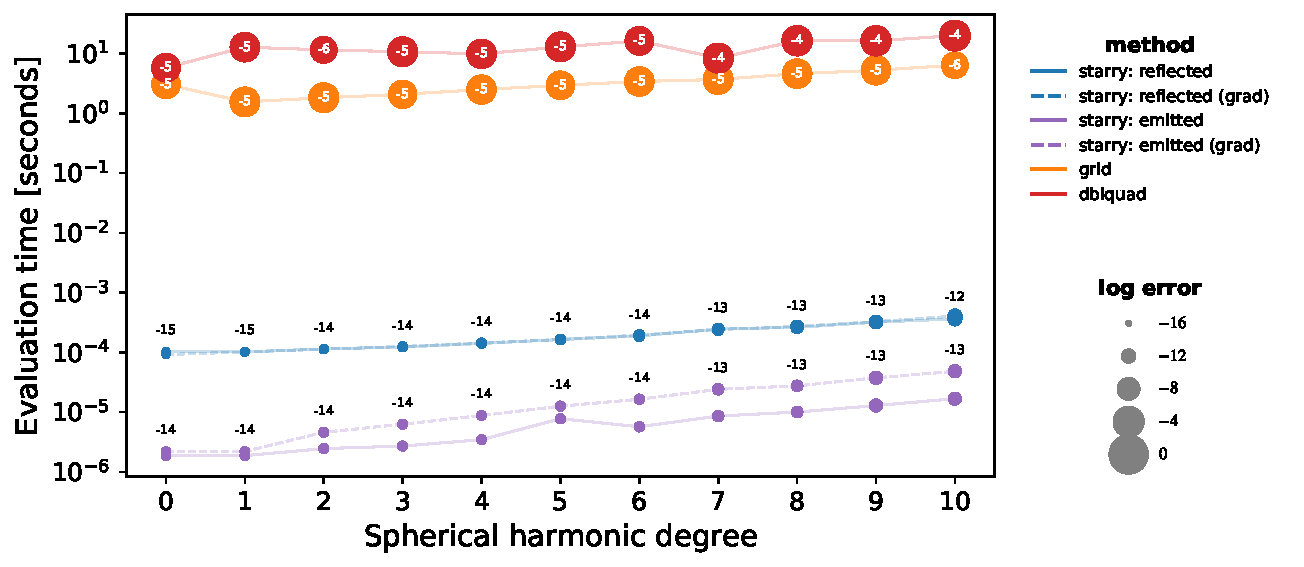
\includegraphics[width=\linewidth]{figures/speed.pdf}
        \oscaption{speed}{%
            Evaluation time for the starry algorithm.
            \label{fig:speed}
        }
    \end{centering}
\end{figure}

\appendix

\xxx{Work in progress below here.}

\section{The \starry formalism}
\label{app:starry}
%
Equations:
%
\begin{align}
    \label{eq:R}
    \BF{R} = ?
\end{align}
%
\begin{align}
    \label{eq:by}
    \by = ?
\end{align}
%
\begin{align}
    \label{eq:bp}
    \bp & =
    \begin{pmatrix}
        1   &
        x   & z  & y  &
        x^2 & xz & xy & yz & y^2 &
        \cdot\cdot\cdot
    \end{pmatrix}^\mathsf{T}
    \quad,
\end{align}
%
\begin{align}
    \label{eq:A1}
    \BF{A_1} = ?
\end{align}
%
\begin{align}
    \label{eq:rTe}
    \rTe = ?
\end{align}
%
\begin{align}
    \label{eq:R'}
    \BF{R}' = ?
\end{align}
%
\begin{align}
    \label{eq:R''}
    \BF{R}'' = ?
\end{align}
%
\begin{align}
    \label{eq:A}
    \BF{A} = ?
\end{align}
%
\begin{align}
    \label{eq:sTe}
    \sTe = ?
\end{align}
%
The basis $\bg$ is called the \emph{Green's basis}; its name
stems from the fact that its components have a structure that makes integration
by Green's theorem convenient. Its components were defined in
Equation~11 of \citet{Luger2019b}:
%
\begin{proof}{bg}
    \tilde{g}_{l,m} &=
    \begin{dcases}
        %
        \frac{\mu+2}{2}x^\frac{\mu}{2} y^\frac{\nu}{2}
         & \qquad \mu, \nu \, \mathrm{even}
        \\[1em]
        %
        z(x, y)
         & \qquad \mu = \nu = 1
        \\[1em]
        %
        3x^{l-2}yz(x, y)
         & \qquad \nu \, \mathrm{odd}, \,
        \mu = 1, \,
        \frac{\mu + \nu}{2} \, \mathrm{even}
        \\[1em]
        %
        z(x, y)
        \bigg(
        -x^{l-3} + x^{l-1} + 4x^{l-3}y^2
        \bigg)
         & \qquad \nu \, \mathrm{odd}, \,
        \mu = 1, \,
        \, \mathrm{odd}
        \\[1em]
        %
        z(x, y)
        \bigg(
        \frac{\mu-3}{2} x^\frac{\mu-5}{2} y^\frac{\nu-1}{2}
        \ - \
        \frac{\mu-3}{2} x^\frac{\mu-5}{2} y^\frac{\nu+3}{2}
        \\
        \qquad\qquad \ - \
        \frac{\mu+3}{2} x^\frac{\mu-1}{2} y^\frac{\nu-1}{2}
        \bigg)
         & \qquad \mathrm{otherwise}
        \quad,
    \end{dcases}
    \label{eq:bg}
\end{proof}
%
where $x$ and $y$ are the Cartesian coordinates on the surface
of the projected
disk of the body, with $z(x, y) = \sqrt{1 - x^2 - y^2}$, and
%
\begin{align}
    \label{eq:munu}
    \mu & = l - m
    \nonumber     \\
    \nu & = l + m
    \quad.
\end{align}
%
The vector $\bg$ is ordered such that
the component at index $n$ is $\tilde{g}_{l,m}$, with
%
\begin{align}
    \label{eq:lm}
    l & = \floor*{\sqrt{n}} \nonumber \\
    m & = n - l^2 - l
    \quad.
\end{align}
%
Finally, the rotation matrix $\BF{R} = \BF{R}(i, \lambda, \vartheta)$
rotates the body to the correct orientation on the sky given its
inclination $i$, obliquity $\lambda$, and rotational phase $\vartheta$,
while $\BF{R}'$ rotates the body on the plane
of the sky into the frame $\mathcal{F}'$ in which the integration is
actually performed, with the occultor along the $+y'$-axis.
For more information on all of these terms, the reader is referred to
\citet{Luger2019}.

The \emph{polynomial basis} $\bp$
\citep[Equation 7 in][]{Luger2019}:
%
\begin{align}
    \tilde{p}_{l,m}(x, y) & =
    \begin{dcases}
        x^\frac{\mu}{2} y^\frac{\nu}{2}
         & \qquad \mu, \nu \, \mathrm{even}
        \\[1em]
        x^\frac{\mu-1}{2} y^\frac{\nu-1}{2} z(x, y)
         & \qquad \mathrm{otherwise} \quad,
    \end{dcases}
\end{align}
%
where $\bp$ is again ordered such that the component at
index $n$ is $\tilde{p}_{l,m}$, with $l$ and $m$ given by
Equation~(\ref{eq:lm}).

As in \citet{Luger2019}, the elements of the solution vector $\mathbf{s}^\top$
are given by the line integral
%
\begin{align}
    \label{eq:s}
    s_{n(\mu,\nu)} = \oint \mathbf{G}_{\mu,\nu} \cdot \dd\mathbf{r}
\end{align}
%
where
%
\begin{align}
    \label{eq:G}
    \BF{G}_{\mu,\nu} (x, y) & =
    \begin{dcases}
        %
        x^{\frac{\mu + 2}{2}}
        y^{\frac{\nu}{2}}
        \,\yhat
         & \qquad \mu, \nu \, \mathrm{even}
        \\[1em]
        %
        \frac{1-z(x, y)^3}{3(1-z(x, y)^2)}\bigg(-y \, \xhat + x \, \yhat\bigg)
         & \qquad \mu = \nu = 1
        \\[1em]
        %
        x^{l-2}
        z(x, y)^3
        \,\xhat
         & \qquad \nu \, \mathrm{odd}, \,
        \mu = 1, \,
        \frac{\mu + \nu}{2} \, \mathrm{even}
        \\[1em]
        %
        x^{l-3}
        y
        z(x, y)^3
        \,\xhat
         & \qquad \nu \, \mathrm{odd}, \,
        \mu = 1, \,
        \frac{\mu + \nu}{2} \, \mathrm{odd}
        \\[1em]
        %
        x^{\frac{\mu-3}{2}}
        y^{\frac{\nu-1}{2}}
        z(x, y)^3
        \,\yhat
         & \qquad \mathrm{otherwise,}
    \end{dcases}
\end{align}
%
and
%
\begin{align}
    \dd \BF{r} & = -r \sin\varphi \, \dd \varphi \, \xhat +
    r \cos\varphi \, \dd \varphi \, \yhat
    \quad,
\end{align}
%
where $\varphi = \varphi(x, y)$ is the parametrized angle along the
arc of integration. Generally, there are at most three arcs bounding a given
closed surface of integration, which we will denote $\mathcal{P}$,
$\mathcal{Q}$, and $\mathcal{T}$. These are shown for a typical
occultor-occulted configuration in Figure~\ref{fig:geometry}.

\subsection{Definitions}
%
Define the pairwise difference operator
%
\begin{align}
    \label{eq:pairdiff}
    \Delta \BS{v} \equiv \sum_{i=0}^{\frac{N - 1}{2}}
    \left( v_{2i + 1} - v_{2i} \right)
\end{align}
%
which sums the difference of successive pairs of values in
an array $\BS{v} = \{ v_0, v_1, v_2, v_3, {\cdot\cdot\cdot}, v_N\}$.

Define the quantity
%
\begin{align}
    \label{eq:q}
    \BS{q}(k^2, \bkappa) = \sqrt{1 - \frac{\sinhalfkap[2]}{k^2}}
    \quad.
\end{align}

\subsection{$\mathcal{H}_{u,v}$}
%
The function $\mathcal{H}_{u,v}$ is given by
%
\begin{align}
    \label{eq:H}
    \mathcal{H}_{u,v}(\blambda) & =
    \lamint{
        \cos^u\varphi
        \sin^v\varphi
    }
    \quad.
\end{align}
%
The integral in this expression is the same as that in Equation (D27)
of \citet{Luger2019}, except for a change in the limits of integration.
We can compute this integral recursively given four lower boundary conditions:
%
\begin{proof}{H}
    \label{eq:Hlower}
    \mathcal{H}_{0,0}(\blambda) &= \Delta \blambda
    %
    \nonumber \\
    %
    \mathcal{H}_{1,0}(\blambda) &= \Delta \sin\blambda
    %
    \nonumber \\
    %
    \mathcal{H}_{0,1}(\blambda) &= -\Delta \cos\blambda
    %
    \nonumber \\
    %
    \mathcal{H}_{1,1}(\blambda) &= -\frac{\Delta\cos^2\blambda}{2}
    %
    \quad.
\end{proof}
%
The remaining terms may be computed by upward recursion using the
relations
%
\begin{proof}{H}
    \label{eq:Hrec1}
    \mathcal{H}_{u,v}(\blambda) &=
    \frac{
        -\Delta \left(
        \cos^{u + 1} \blambda
        \sin^{v - 1} \blambda
        \right)
        +(v - 1)\mathcal{H}_{u,v - 2}(\blambda)
    }{u + v}
\end{proof}
%
for $u < 2, v \ge 2$ and
%
\begin{proof}{H}
    \label{eq:Hrec2}
    \mathcal{H}_{u,v}(\blambda) &=
    \frac{
        \Delta \left(
        \cos^{u - 1} \blambda
        \sin^{v + 1} \blambda
        \right)
        + (u - 1)\mathcal{H}_{u - 2,v}(\blambda)
    }{u + v}
\end{proof}
%
for all remaining terms.

\subsection{$\mathcal{T}_{2}$}
%
The function $\mathcal{T}_{2}$ is given by
%
\begin{align}
    \label{eq:T2}
    \mathcal{T}_{2}(b, \bxi) & = ?
    \quad.
\end{align}

\begin{proof}{}
    \mathcal{T}_{2}(b, \bxi) &= -\sgn(b) \Delta \BS{f}(b, \bxi)
\end{proof}
%
where
%
\begin{proof}{}
    \begin{split}
        f_i(b, \xi_i) =
        \frac{1}{3}\scalebox{1.4}{\Bigg(}
        &\arctan\left( \frac{|b|\sin\xi_i}{\cos\xi_i} \right)
        %
        \\
        %
        &- \sgn\left({\sin\xi_i}\right)
        \left(
        \arctan
        \left(
            \frac{
                \left(\frac{\sin\xi_i}{1 + \cos\xi_i}\right)^2 + 2 b^2 - 1
            }{2 |b| \sqrt{1 - b^2}}
            \right)
        + |b| \sqrt{1 - b^2} \cos\xi_i
        \right)
        %
        \\
        %
        &+ \phi(b, \xi_i)
        \scalebox{1.4}{\Bigg)}
    \end{split}
\end{proof}
%
and
%
\begin{proof}{}
    \phi(b, \xi_i) & =
    \begin{cases}
        0                          & \qquad 0 \leq \xi_i < \frac{\pi}{2}     \\
        \pi                        & \qquad \frac{\pi}{2} \leq \xi_i < \pi   \\
        2 |b| \sqrt{1 - b^2}       & \qquad \pi < \xi_i \leq \frac{3\pi}{2}  \\
        \pi + 2 |b| \sqrt{1 - b^2} & \qquad \frac{3\pi}{2} \leq \xi_i < 2\pi
        \quad.
    \end{cases}
\end{proof}

\subsection{$\mathcal{U}_v$}
%
The function $\mathcal{U}_v$ is given by
%
\begin{align}
    \label{eq:U}
    \mathcal{U}_v(\bkappa) =
    \kapint{\cos\varphi\sin^{2v}\varphi}
    \quad.
\end{align}
%
This integral has an analytic solution for all $v$:
%
\begin{proof}{U}
    \label{eq:Usol}
    \mathcal{U}_v(\bkappa) &= \frac{\Delta \sinhalfkap[v+1]}{v + 1}
    \quad.
\end{proof}
%

\subsection{$\mathcal{I}_v$}
%
The function $\mathcal{I}_v$ is given by
%
\begin{align}
    \label{eq:I}
    \mathcal{I}_v(\bkappa) & =
    \kapint{\sinhalfkap[2v]}
    \quad.
\end{align}
%
The integral in this expression is the same as that in Equation (D38)
of \citet{Luger2019}, except for a change in the limits of integration.
As in \citet{Luger2019}, we can compute this integral recursively given
a trivial lower boundary condition:
%
\begin{proof}{I}
    \label{eq:Irec}
    \mathcal{I}_0(\bkappa) &=
    \frac{\Delta \bkappa}{2}
    %
    \nonumber \\
    %
    \mathcal{I}_v(\bkappa) &=
    \frac{1}{2v}
    \bigg(
    (2v - 1) \mathcal{I}_{v-1}(\bkappa) -
    \Delta \left(\sinhalfkap[2v - 1]\coshalfkap\right)
    \bigg)
\end{proof}
%
where the last expression is valid for all $v > 0$. We find that this algorithm
is generally stable, except when $\sin\left(\frac{\bkappa}{2}\right)$ is small.
In that limit, we evaluate $\mathcal{I}_N(\bkappa)$ by numerical integration of
Equation~(\ref{eq:I}) using Gauss-Legendre quadrature with \STARRYQUADPOINTS
points. We then recurse downward by substituting $v \rightarrow v + 1$ in
Equation~(\ref{eq:Irec}) and solving for $\mathcal{I}_v(\bkappa)$.

\subsection{$\mathcal{J}_v$}
%
The function $\mathcal{J}_v$ is given by
%
\begin{align}
    \label{eq:J}
    \mathcal{J}_v(k^2, \bkappa) =
    \kapint{
        \sin^{2v}\varphi
        \left(1 - \frac{\sin^2\varphi}{k^2}\right)^\frac{3}{2}
    }
    \quad.
\end{align}
%
The integral in this expression is again the same as that in Equation (D39)
of \citet{Luger2019}, except for a change in the limits of integration.
In that paper, we computed all terms
$\{ \mathcal{J}_0, {\cdot\cdot\cdot}, \mathcal{J}_\vmax \}$ from a three-term
recurrence relation and two boundary conditions. In the case of upward
recursion, the boundary conditions $\mathcal{J}_0$ and $\mathcal{J}_1$ were
computed analytically from the complete elliptic integrals $K(k^2)$
and $E(k^2)$. In cases where upward recursion was not numerically stable, we
evaluated $\mathcal{J}_\vmax$ and $\mathcal{J}_{\vmax-1}$
via a quickly convergent series expansion and recursed downward.

In order to solve Equation~(\ref{eq:J}), it is possible to
replace the complete elliptic integrals $K(k^2)$ and $E(k^2)$ in the lower
boundary conditions \citep[Equation D46 in ][]{Luger2019} with the
incomplete elliptic integrals $F(k^2, \kappa)$ and $E(k^2, \kappa)$,
then use the same upward
recursion relation to obtain analytic solutions for all $\mathcal{J}_v$:
%
\begin{proof}{J}
    \label{eq:Jrec}
    \mathcal{J}_0(k^2, \bkappa) &=
    \frac{1}{3} \bigg(
    2 \left(2 - \frac{1}{k^2}\right) \DE +
    \left(\frac{1}{k^2} - 1\right) \DF +
    \Delta \BS{z}_0(k^2, \bkappa)
    \bigg)
    %
    \nonumber \\
    %
    \mathcal{J}_1(k^2, \bkappa) &=
    \frac{1}{15} \bigg(
    \left(-3 k^2 + 13 - \frac{8}{k^2}\right) \DE +
    \left(3 k^2 - 7 + \frac{4}{k^2}\right) \DF +
    \Delta \BS{z}_1(k^2, \bkappa)
    \bigg)
    %
    \nonumber \\
    %
    \mathcal{J}_v(k^2, \bkappa) &=
    \frac{1}{2v + 3}
    \bigg(
    2 \left( v + 1 + (v - 1) k^2 \right) \mathcal{J}_{v - 1} -
    (2v - 3) k^2 \mathcal{J}_{v - 2}
    + \Delta \BS{z}_v(k^2, \bkappa)
    \bigg)
\end{proof}
%
%
where the last expression is valid for all $v > 1$ and
%
\begin{proof}{J}
    \label{eq:Jrec_z}
    \BS{z}_0(k^2, \BS{\kappa}) & =
    \frac{
        \sinhalfkap
        \coshalfkap
        \BS{q}(k^2, \bkappa)
    }{
        k^2
    }
    %
    \nonumber\\
    %
    \BS{z}_1(k^2, \BS{\kappa}) & =
    \left(\left(3 \sinhalfkap[2] + 4\right) - 6k^2\right)
    \BS{z}_0(k^2, \BS{\kappa})
    %
    \nonumber\\
    %
    \BS{z}_v(k^2, \BS{\kappa}) & =
    k^2
    \sinhalfkap[2v - 3]
    \coshalfkap
    \BS{q}(k^2, \BS{\kappa})^5
    \quad.
\end{proof}
%
However, in practice we find that this procedure is even more numerically
unstable than it was in \citet{Luger2019}.
To address this, we express the recurrence structure of the problem as
a tridiagonal system with one lower boundary condition $\mathcal{J}_0$
and one upper boundary condition $\mathcal{J}_\vmax$:
%
\begin{proof}{J}
    \label{eq:Jtri}
    \begin{pmatrix}
        a_0 & 1   &     &        &         &         \\
        b_1 & a_1 & 1   &        &         &         \\
            & b_2 & a_2 & 1      &         &         \\
            &     & b_0 & a_3    & 1       &         \\
            &     &     & \ddots & \ddots  & \ddots  \\
            &     &     &        & b_\vmax & a_\vmax
    \end{pmatrix}
    \begin{pmatrix}
        \mathcal{J}_1   \\
        \mathcal{J}_2   \\
        \mathcal{J}_3   \\
        \mathcal{J}_4   \\
        \cdot\cdot\cdot \\
        \mathcal{J}_{\vmax-1}
    \end{pmatrix}
    =
    \begin{pmatrix}
        c_0 - b_0 \mathcal{J}_0 \\
        c_1                     \\
        c_2                     \\
        c_3                     \\
        \cdot\cdot\cdot         \\
        c_\vmax - \mathcal{J}_\vmax
    \end{pmatrix}
\end{proof}
%
where the recursion coefficients are given by
%
\begin{proof}{J}
    \label{eq:Jtri_coeffs}
    a_v(k) &= -2\frac{(v + 1) + (v - 1) k^2}{2v + 3} \nonumber \\
    b_v(k) &= \frac{(2v - 3) k^2}{2v + 3} \nonumber \\
    c_v(k^2, \bkappa) &= \Delta
    \bigg(
    \frac{
            \BS{z}_v(k^2, \BS{\kappa})
        }{
            2v + 3
        }
    \bigg)
    \quad.
\end{proof}
%
Solving this matrix system yields values for all
intermediate $\{ \mathcal{J}_1, {\cdot\cdot\cdot}, \mathcal{J}_{\vmax - 1} \}$.
While efficient algorithms exist for solving tridiagonal problems, we obtain
far better numerical stability by instead performing traditional LU
decomposition. We find that this algorithm is stable in all the regimes that we
tested.

We evaluate the upper boundary condition $\mathcal{J}_{\vmax}$ by numerical
integration of Equation~(\ref{eq:J}) via Gauss-Legendre quadrature with
\STARRYQUADPOINTS points. While the lower boundary condition may be computed
analytically from Equation~(\ref{eq:Jrec}),
in practice we achieve better precision via numerical
integration (as above), with negligible effects on computational performance.

\subsection{$\mathcal{W}_n$}
%
The function $\mathcal{W}_n$ is given by
%
\begin{align}
    \label{eq:W}
    % TODO
    \mathcal{W}_n = \int
\end{align}
%
This integral has a closed-form solution:
%
\begin{proof}{}
    \label{eq:Wsol}
    \mathcal{W}_n =
    \frac{\sin^{2n + 2}\left(\frac{\bkappa}{2}\right)}{2n + 5}
    \left(
    \frac{3}{n+1}
        {_2F_1}\left(-\frac{1}{2}, n + 1; n + 2; 1 - q^2\right) + 2 q^3
    \right)
\end{proof}
%
where ${_2F_1}(a, b; c; z)$ is the Gauss hypergeometric function.


% by either upward recursion (stable for |1 - q^2| > 1/2) or downward
% recursion (always stable).

% Bibliography
\bibliography{bib}


\end{document}
